\documentclass[12pt, a4paper]{article}
\usepackage[margin=0.5in]{geometry}

\usepackage{color}
\usepackage[dvipsnames]{xcolor}
\usepackage{hyperref}
\hypersetup{
    colorlinks=true,
    linkcolor=blue,
    urlcolor=blue,
    linktoc=all
}


\usepackage{amsmath}
\usepackage{mathtools}
\usepackage{amssymb}
\usepackage{cancel}
\usepackage{bm}
\usepackage{dsfont}
\usepackage{graphicx}
\usepackage{graphics}
\usepackage{xfrac}
\usepackage{array}
\setcounter{MaxMatrixCols}{40}

\usepackage{enumerate}
\usepackage{enumitem}
\usepackage{multirow}

%inclusions carried over from past class homework formats
\usepackage{units}
\usepackage{fullpage}
\usepackage{alltt}
\usepackage{mathrsfs}
\usepackage{xcolor}
\usepackage{soul}

\usepackage{pgfplots}

\DeclarePairedDelimiter{\abs}{\lvert}{\rvert}
\newcommand*{\fontCourier}{\fontfamily{pcr}\selectfont}
\newcommand*\mean[1]{\overline{#1}}
\newcommand\scalemath[2]{\scalebox{#1}{\mbox{\ensuremath{\displaystyle #2}}}}

\setcounter{tocdepth}{5}
\setcounter{secnumdepth}{5}

\usepackage{pdfpages}
\usepackage{Sweave}
\begin{document}
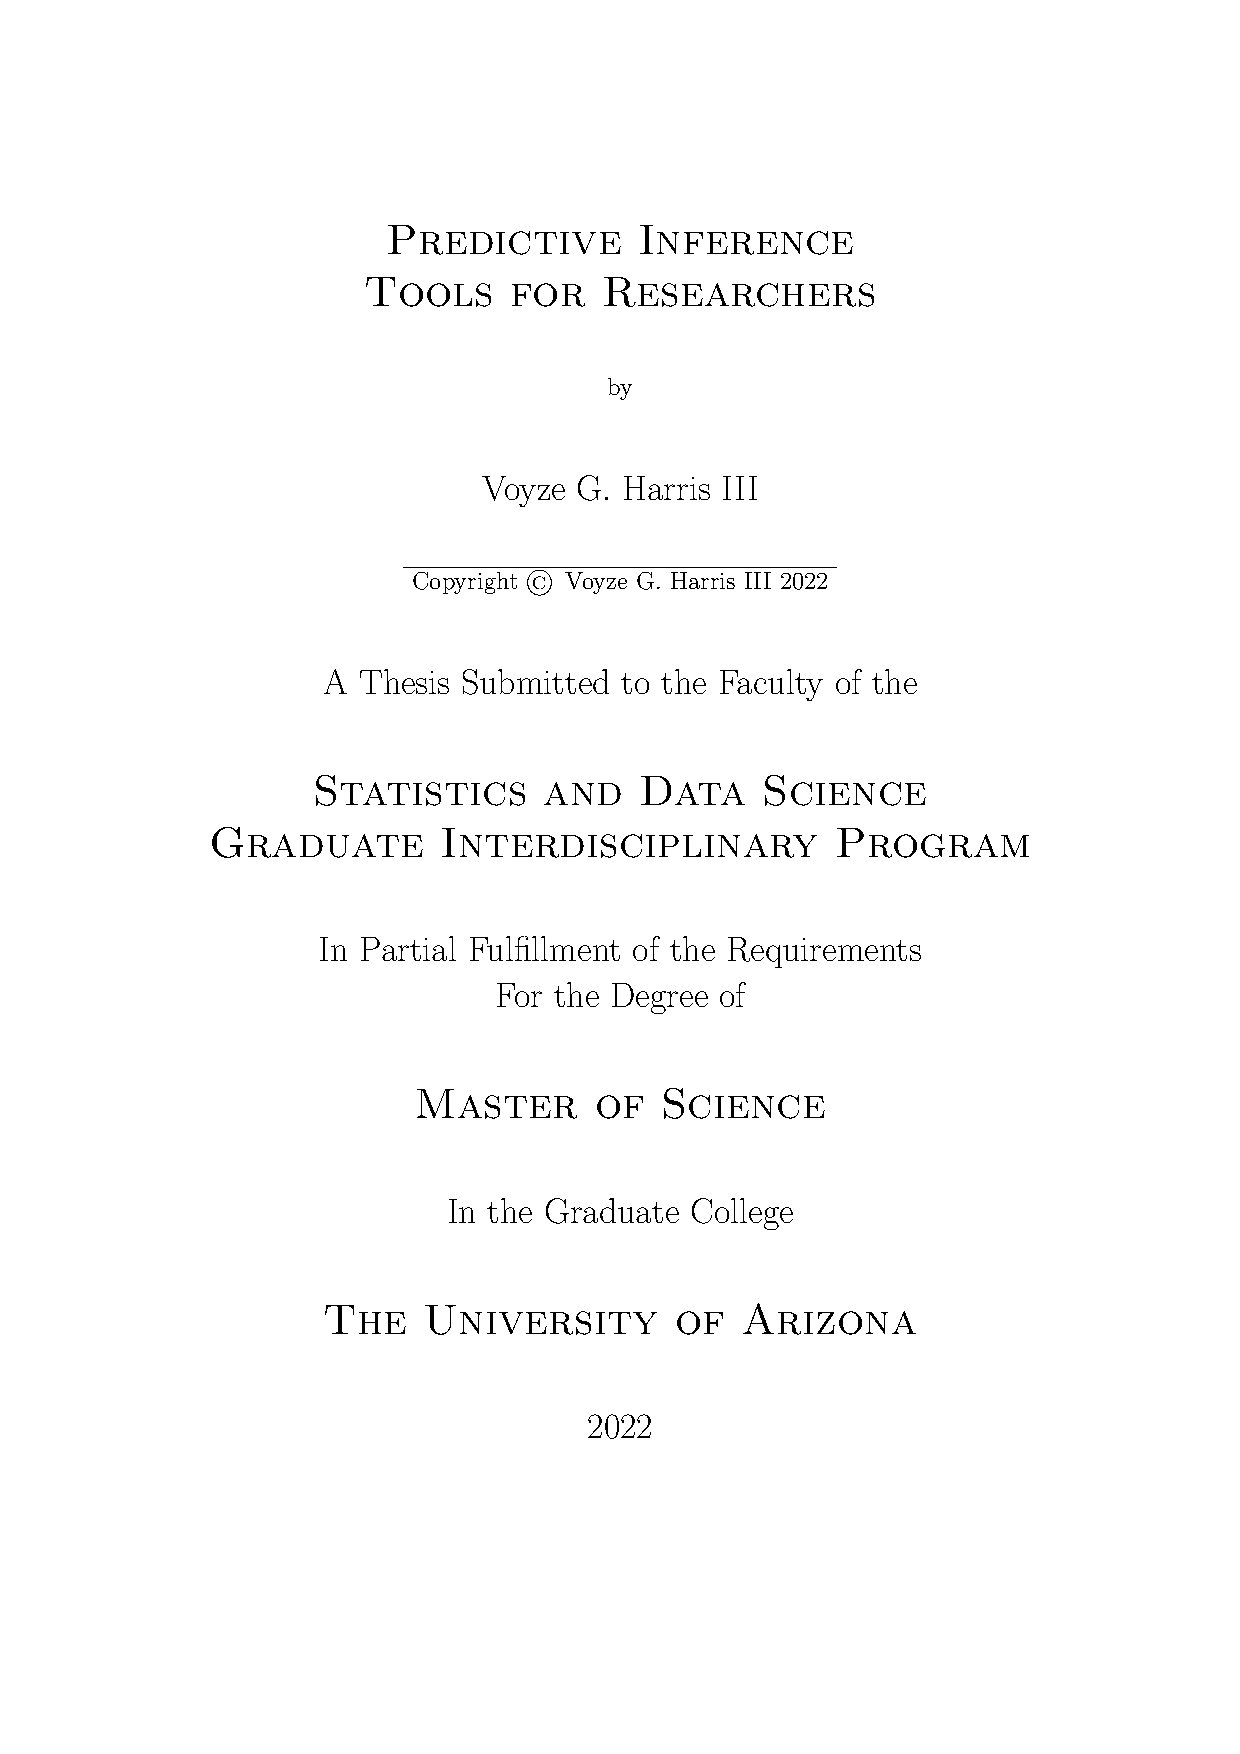
\includepdf{TitlePage_MastersThesis}

\includepdf{ThesisApprovalPage}
\Sconcordance{concordance:Thesis.tex:Thesis.Rnw:%
1 49 1 1 0 7 1 1 4 99 1 1 31 1 12 69 1 1 45 1 2 179 1 1 46 1 2 120 1 1 %
23 7 0 1 76 4 0 1 5 32 1 1 26 1 4 26 1}


\tableofcontents
\newpage


%%%%%%%%%%%%%%%%%%%%%%%%%%%%%%%%%
%%INTRODUCTION
%%%%%%%%%%%%%%%%%%%%%%%%%%%%%%%%%
\section{Thesis Abstract}
  \begin{itemize}
    \item (paragraph) Statement of the thesis topic and objectives
    \item (paragraph) Explanation of R package
  \end{itemize}

\clearpage

\section{Introduction:  Predictive Inference}

  \subsection{Why is predictive inference important?}

  \subsection{Difference between parametric inference and predictive inference}

    \subsubsection{When is predictive inference more useful?}

    \subsubsection{When is parametric inference more useful?}
      [examples, comparisons]

  \subsection{The Bayesian Parametric Prediction Format}
    [Geisser p. 49]\\

        Let $$f\left(x^{(N)},x_{(M)}|\theta\right) = f\left(x_{(M)}|x^{(N)},\theta\right)f\left(x^{(N)}|\theta\right).$$

    Here $x^{(N)}$ represents observed events and $x_{(M)}$ are future events.  We calculate

    $$f\left(x_{(M)},x^{(N)}\right) = \int f\left(x^{(N)},x_{(M)}|\theta\right)p(\theta)d\theta$$

    where $p(\theta)$ is the prior density and

    $$f\left(x_{(M)}|x^{(N)}\right) = \frac{f\left(x_{(M)},x^{(N)}\right)}{f\left(x^{(N)}\right)} = \int f\left(x_{(M)}|\theta\right)p\left(\theta|x^{(N)}\right)d\theta$$

    where

    $$p\left(\theta|x^{(N)}\right) \propto f\left(x^{(N)}|\theta\right)p(\theta).$$

  \subsection{[Maybe] Example of Difference between results from Plug-in estimator and results using Predictive Inference}

\clearpage

\section{Chapter 1:  Predictive Problems with Conjugate Priors}

  [Problems with closed-form solutions.  These problems will be what the R package is designed for.  Use problems from Geisser, Casella \& Berger (Bayesian chapter), other sources.  Regression problem--predictive distributions of models that include and exclude some predictor]

  \subsection{Prediction of Future Successes:  Beta-Binomial (Geisser p. 73)}


    \subsubsection{Derivation}

      Let $X_i$ be independent binary variables with Pr$(X_i = 1) = \theta$, and let $T = \sum X_i$.  Then $T$ has probability

      $${N\choose t}\theta^t(1-\theta)^{N-t}.$$

      \vspace{5mm}

      Assume $\theta\sim\text{Beta}(\alpha,\beta)$, so

      \vspace{5mm}

      $$p(\theta) = \frac{\Gamma(\alpha + \beta)\theta^{\alpha - 1}(1 - \theta)^{\beta - 1}}{\Gamma(\alpha)\Gamma(\beta)}.$$

      \vspace{5mm}

      Then

      \vspace{5mm}

      $$p\left(\theta|X^{(N)}\right) = \frac{\Gamma(N+\alpha+\beta)\theta^{t+\alpha-1}(1-\theta)^{N-t+\beta-1}}{\Gamma(t+\alpha)\Gamma(N-t+\beta)}$$

      \vspace{5mm}

      \noindent So for $R = \sum_{i=1}^M X_{N+i}$ we have Beta-Binomial predictive distribution

\begin{flalign*}
  \text{Pr}[R=r|t]
  &= \int {M\choose r}\theta^r(1-\theta)^{M-r}p\left(\theta|X^{(N)}\right)d\theta\\
  &\\
  &= {M\choose r}\int \theta^r(1-\theta)^{M-r}\frac{\Gamma(N+\alpha+\beta)}{\Gamma(t+\alpha)\Gamma(N-t+\beta)}\theta^{t+\alpha-1}(1-\theta)^{N-t+\beta-1}d\theta\\
  &\\
  &= \frac{M!}{r!(M-r)!}\frac{\Gamma(N+\alpha+\beta)}{\Gamma(t+\alpha)\Gamma(N-t+\beta)}\int\theta^{r+t+\alpha-1}(1-\theta)^{M-r+N-t+\beta-1}d\theta\\
  &\\
  &= \frac{\Gamma(M+1)\Gamma(N+\alpha+\beta)\Gamma(r+t+\alpha)\Gamma(M-r+N-t+\beta)}{\Gamma(r+1)\Gamma(M-r+1)\Gamma(t+\alpha)\Gamma(N-t+\beta)\Gamma(M+N+\alpha+\beta)}
\end{flalign*}

\clearpage

    \subsubsection{R Implementation}

This result has been used to create ``standard" R functions dpredBB(), ppredBB(), and rpredBB() for the Beta-Binomial distribtuion for density, cumulative probability, and random sampling, respectively (see appendix).  These functions are exercised in the following example.


    \subsubsection{Example}

Suppose $t=5$ successes have been observed out of $N=10$ binary events, $\alpha = 2$ and $\beta = 8$.  For $M = 1000$ future observations, the figures below show the predictive distribution from dpredBB(), the cumulative distribution from ppredBB(), and a histogram of random draws from rpredBB().


